% Options for packages loaded elsewhere
\PassOptionsToPackage{unicode}{hyperref}
\PassOptionsToPackage{hyphens}{url}
\PassOptionsToPackage{dvipsnames,svgnames,x11names}{xcolor}
%
\documentclass[
  letterpaper,
  DIV=11,
  numbers=noendperiod]{scrartcl}

\usepackage{amsmath,amssymb}
\usepackage{iftex}
\ifPDFTeX
  \usepackage[T1]{fontenc}
  \usepackage[utf8]{inputenc}
  \usepackage{textcomp} % provide euro and other symbols
\else % if luatex or xetex
  \usepackage{unicode-math}
  \defaultfontfeatures{Scale=MatchLowercase}
  \defaultfontfeatures[\rmfamily]{Ligatures=TeX,Scale=1}
\fi
\usepackage{lmodern}
\ifPDFTeX\else  
    % xetex/luatex font selection
\fi
% Use upquote if available, for straight quotes in verbatim environments
\IfFileExists{upquote.sty}{\usepackage{upquote}}{}
\IfFileExists{microtype.sty}{% use microtype if available
  \usepackage[]{microtype}
  \UseMicrotypeSet[protrusion]{basicmath} % disable protrusion for tt fonts
}{}
\makeatletter
\@ifundefined{KOMAClassName}{% if non-KOMA class
  \IfFileExists{parskip.sty}{%
    \usepackage{parskip}
  }{% else
    \setlength{\parindent}{0pt}
    \setlength{\parskip}{6pt plus 2pt minus 1pt}}
}{% if KOMA class
  \KOMAoptions{parskip=half}}
\makeatother
\usepackage{xcolor}
\setlength{\emergencystretch}{3em} % prevent overfull lines
\setcounter{secnumdepth}{-\maxdimen} % remove section numbering
% Make \paragraph and \subparagraph free-standing
\ifx\paragraph\undefined\else
  \let\oldparagraph\paragraph
  \renewcommand{\paragraph}[1]{\oldparagraph{#1}\mbox{}}
\fi
\ifx\subparagraph\undefined\else
  \let\oldsubparagraph\subparagraph
  \renewcommand{\subparagraph}[1]{\oldsubparagraph{#1}\mbox{}}
\fi


\providecommand{\tightlist}{%
  \setlength{\itemsep}{0pt}\setlength{\parskip}{0pt}}\usepackage{longtable,booktabs,array}
\usepackage{calc} % for calculating minipage widths
% Correct order of tables after \paragraph or \subparagraph
\usepackage{etoolbox}
\makeatletter
\patchcmd\longtable{\par}{\if@noskipsec\mbox{}\fi\par}{}{}
\makeatother
% Allow footnotes in longtable head/foot
\IfFileExists{footnotehyper.sty}{\usepackage{footnotehyper}}{\usepackage{footnote}}
\makesavenoteenv{longtable}
\usepackage{graphicx}
\makeatletter
\def\maxwidth{\ifdim\Gin@nat@width>\linewidth\linewidth\else\Gin@nat@width\fi}
\def\maxheight{\ifdim\Gin@nat@height>\textheight\textheight\else\Gin@nat@height\fi}
\makeatother
% Scale images if necessary, so that they will not overflow the page
% margins by default, and it is still possible to overwrite the defaults
% using explicit options in \includegraphics[width, height, ...]{}
\setkeys{Gin}{width=\maxwidth,height=\maxheight,keepaspectratio}
% Set default figure placement to htbp
\makeatletter
\def\fps@figure{htbp}
\makeatother

\usepackage[auth-lg]{authblk}
\KOMAoption{captions}{tableheading}
\makeatletter
\makeatother
\makeatletter
\makeatother
\makeatletter
\@ifpackageloaded{caption}{}{\usepackage{caption}}
\AtBeginDocument{%
\ifdefined\contentsname
  \renewcommand*\contentsname{Table of contents}
\else
  \newcommand\contentsname{Table of contents}
\fi
\ifdefined\listfigurename
  \renewcommand*\listfigurename{List of Figures}
\else
  \newcommand\listfigurename{List of Figures}
\fi
\ifdefined\listtablename
  \renewcommand*\listtablename{List of Tables}
\else
  \newcommand\listtablename{List of Tables}
\fi
\ifdefined\figurename
  \renewcommand*\figurename{Figure}
\else
  \newcommand\figurename{Figure}
\fi
\ifdefined\tablename
  \renewcommand*\tablename{Table}
\else
  \newcommand\tablename{Table}
\fi
}
\@ifpackageloaded{float}{}{\usepackage{float}}
\floatstyle{ruled}
\@ifundefined{c@chapter}{\newfloat{codelisting}{h}{lop}}{\newfloat{codelisting}{h}{lop}[chapter]}
\floatname{codelisting}{Listing}
\newcommand*\listoflistings{\listof{codelisting}{List of Listings}}
\makeatother
\makeatletter
\@ifpackageloaded{caption}{}{\usepackage{caption}}
\@ifpackageloaded{subcaption}{}{\usepackage{subcaption}}
\makeatother
\makeatletter
\@ifpackageloaded{tcolorbox}{}{\usepackage[skins,breakable]{tcolorbox}}
\makeatother
\makeatletter
\@ifundefined{shadecolor}{\definecolor{shadecolor}{rgb}{.97, .97, .97}}
\makeatother
\makeatletter
\makeatother
\makeatletter
\makeatother
\ifLuaTeX
  \usepackage{selnolig}  % disable illegal ligatures
\fi
\IfFileExists{bookmark.sty}{\usepackage{bookmark}}{\usepackage{hyperref}}
\IfFileExists{xurl.sty}{\usepackage{xurl}}{} % add URL line breaks if available
\urlstyle{same} % disable monospaced font for URLs
\hypersetup{
  pdftitle={Análise parlamentares},
  colorlinks=true,
  linkcolor={blue},
  filecolor={Maroon},
  citecolor={Blue},
  urlcolor={Blue},
  pdfcreator={LaTeX via pandoc}}

\title{Análise parlamentares}
\usepackage{etoolbox}
\makeatletter
\providecommand{\subtitle}[1]{% add subtitle to \maketitle
  \apptocmd{\@title}{\par {\large #1 \par}}{}{}
}
\makeatother
\subtitle{Cliente: Isabela (\ldots)}
\author{}
\date{}

\begin{document}
\maketitle
\ifdefined\Shaded\renewenvironment{Shaded}{\begin{tcolorbox}[breakable, frame hidden, interior hidden, boxrule=0pt, borderline west={3pt}{0pt}{shadecolor}, enhanced, sharp corners]}{\end{tcolorbox}}\fi

\renewcommand*\contentsname{Table of contents}
{
\hypersetup{linkcolor=}
\setcounter{tocdepth}{2}
\tableofcontents
}
\newpage{}

\hypertarget{descriuxe7uxe3o-geral}{%
\section{Descrição geral}\label{descriuxe7uxe3o-geral}}

Dados disponíveis via API:
\url{https://legis.senado.leg.br/dadosabertos/docs/resource_ListaSenadorService.html}

Em todos os pontos, fazer a análise global (46ª à 56ª legislatura e
legislaturas isoladamente), seguidas de gráficos.

\hypertarget{anuxe1lise-1-paralelo-de-proporuxe7uxe3o-entre-mulheres-e-homens-total}{%
\section{Análise 1: Paralelo de proporção entre mulheres e homens
total}\label{anuxe1lise-1-paralelo-de-proporuxe7uxe3o-entre-mulheres-e-homens-total}}

Número de homens e mulheres (eleitos e suplentes) da 46 à 56ª
legislatura.

Filtrando para casos em que o nome não é \texttt{NA}, perde-se 1309
observações. Saimos de 4094 para 2785 casos. Após a filtragem, a
legislatura mais antiga que se tem é a 48 e a mais recente é a 56.

\begin{longtable}{ccccc}
\caption{Tabela com totais e proporções de sexos entre legislaturas 48 e 56.}\tabularnewline

\toprule
Legislatura & T. Masc. & T. Fem. & Prop. Masc. & Prop. Fem.\\
\midrule
48 & 16 & 0 & 0.00\% & 100.00\%\\
49 & 138 & 7 & 5.07\% & 94.93\%\\
50 & 301 & 22 & 7.31\% & 92.69\%\\
51 & 270 & 22 & 8.15\% & 91.85\%\\
52 & 331 & 36 & 10.88\% & 89.12\%\\
53 & 365 & 39 & 10.68\% & 89.32\%\\
54 & 378 & 39 & 10.32\% & 89.68\%\\
55 & 378 & 38 & 10.05\% & 89.95\%\\
56 & 331 & 74 & 22.36\% & 77.64\%\\
\bottomrule
\end{longtable}

Observamos a presença feminina nas séries temporais a seguir:

\begin{figure}

{\centering 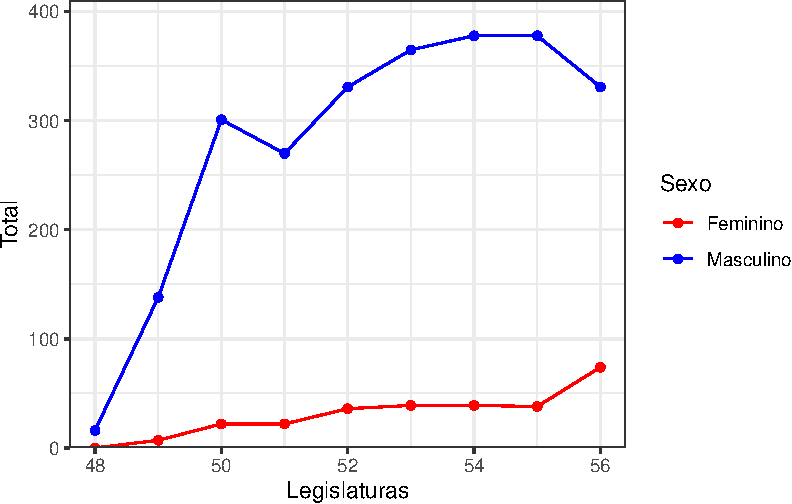
\includegraphics[width=0.75\textwidth,height=\textheight]{caderno-isabela_files/figure-pdf/plot-totais-parlamentares-1.pdf}

}

\caption{Série temporal de totais de parlamentares agrupados por sexo.}

\end{figure}

\begin{figure}

{\centering 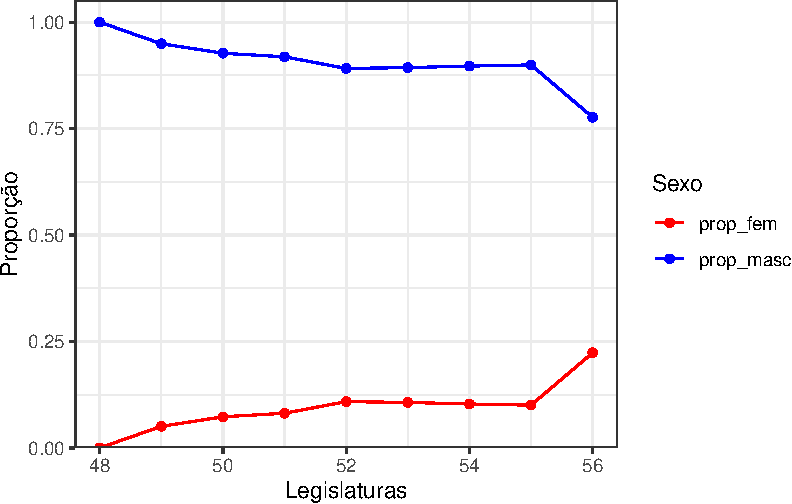
\includegraphics[width=0.75\textwidth,height=\textheight]{caderno-isabela_files/figure-pdf/plot-percentuais-parlamentares-1.pdf}

}

\caption{Série temporal de percentual do total de parlamentares
agrupados por sexo.}

\end{figure}

\begin{figure}

{\centering 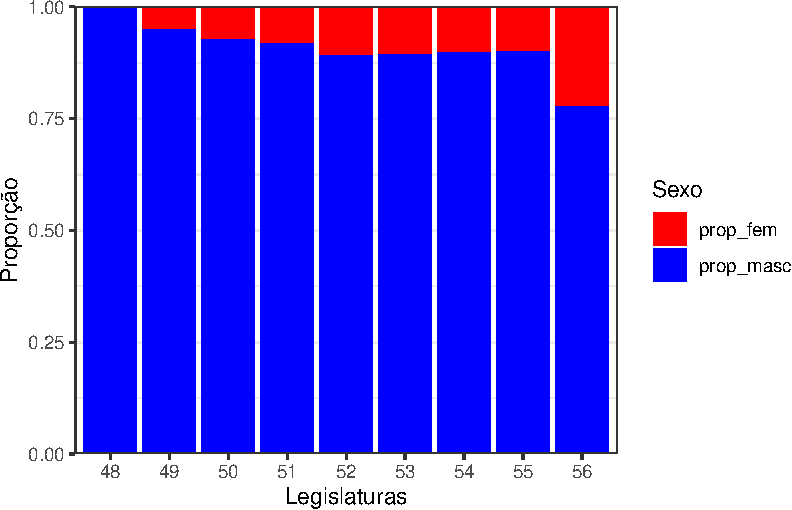
\includegraphics[width=0.75\textwidth,height=\textheight]{caderno-isabela_files/figure-pdf/plot-percentuais-parlamentares-alt-1.pdf}

}

\caption{Série temporal de percentual do total de parlamentares
agrupados por sexo. Visualização alternativa}

\end{figure}

\newpage{}

\hypertarget{anuxe1lise-2-pls-e-ec}{%
\section{Análise 2: PLS e EC}\label{anuxe1lise-2-pls-e-ec}}

AUTORIAS INDIVIDUAIS PLS E EC EM NÚMEROS ABSOLUTOS AUTORIAS INDIVIDUAIS
PLS E EC \% COMPARATIVAMENTE

PL E EC REJEITADAS NO SF EM NÚMEROS ABSOLUTOS PL E EC REJEITADAS NO SF
\% COMPARATIVAMENTE

PL E EC APROVADOS NO SF EM NÚMEROS ABSOLUTOS PL E EC APROVADAS O SF \%
COMPARATIVAMENTE

PL E EC ARQUIVADAS EM NÚMEROS ABSOLUTOS PL E EC ARQUIVADAS
COMPARATIVAMENTE

PL E EC APROVADAS NAS DUAS CASAS E ENCAMINHADAS À SANÇÃO EM NÚMEROS
ABSOLUTOS PL E EC APROVADAS NAS DUAS CASAS E ENCAMINHADAS À SANÇÃO \%
COMPARATIVAMENTE

\newpage{}

\hypertarget{anuxe1lise-3-relatorias}{%
\section{Análise 3: Relatorias}\label{anuxe1lise-3-relatorias}}

RELATORIAS INDIVIDUAIS EM NÚMEROS ABSOLUTOS RELATORIAS INDIVIDUAIS \%
COMPARATIVAMENTE

\newpage{}

\hypertarget{anuxe1lise-4-interrupuxe7uxf5es}{%
\section{Análise 4 --
interrupções}\label{anuxe1lise-4-interrupuxe7uxf5es}}

Aqui, eu não sei se é possível medir as interrupções. No webservice, vi
que disponibilizam discursos, apartes e outros tipos de uso da palavra.
O contraste comparativo e absoluto desse tipo de dados também seria
interessante.



\end{document}
